\documentclass[12pt,a4paper]{article}

%\usepackage[left=1.5cm,right=1.5cm,top=1cm,bottom=2cm]{geometry}
\usepackage[in, plain]{fullpage}
\usepackage{array}
\usepackage{../../../pas-math}
\usepackage{../../../moncours}


%\usepackage{pas-cours}
%-------------------------------------------------------------------------------
%          -Packages nécessaires pour écrire en Français et en UTF8-
%-------------------------------------------------------------------------------
\usepackage[utf8]{inputenc}
\usepackage[frenchb]{babel}
\usepackage[T1]{fontenc}
\usepackage{lmodern}
\usepackage{textcomp}



%-------------------------------------------------------------------------------

%-------------------------------------------------------------------------------
%                          -Outils de mise en forme-
%-------------------------------------------------------------------------------
\usepackage{hyperref}
\hypersetup{pdfstartview=XYZ}
%\usepackage{enumerate}
\usepackage{graphicx}
\usepackage{multicol}
\usepackage{tabularx}
\usepackage{multirow}


\usepackage{anysize} %%pour pouvoir mettre les marges qu'on veut
%\marginsize{2.5cm}{2.5cm}{2.5cm}{2.5cm}

\usepackage{indentfirst} %%pour que les premier paragraphes soient aussi indentés
\usepackage{verbatim}
\usepackage{enumitem}
\usepackage[usenames,dvipsnames,svgnames,table]{xcolor}

\usepackage{variations}

%-------------------------------------------------------------------------------


%-------------------------------------------------------------------------------
%                  -Nécessaires pour écrire des mathématiques-
%-------------------------------------------------------------------------------
\usepackage{amsfonts}
\usepackage{amssymb}
\usepackage{amsmath}
\usepackage{amsthm}
\usepackage{tikz}
\usepackage{xlop}
%-------------------------------------------------------------------------------



%-------------------------------------------------------------------------------


%-------------------------------------------------------------------------------
%                    - Mise en forme avancée
%-------------------------------------------------------------------------------

\usepackage{ifthen}
\usepackage{ifmtarg}


\newcommand{\ifTrue}[2]{\ifthenelse{\equal{#1}{true}}{#2}{$\qquad \qquad$}}

%-------------------------------------------------------------------------------

%-------------------------------------------------------------------------------
%                     -Mise en forme d'exercices-
%-------------------------------------------------------------------------------
%\newtheoremstyle{exostyle}
%{\topsep}% espace avant
%{\topsep}% espace apres
%{}% Police utilisee par le style de thm
%{}% Indentation (vide = aucune, \parindent = indentation paragraphe)
%{\bfseries}% Police du titre de thm
%{.}% Signe de ponctuation apres le titre du thm
%{ }% Espace apres le titre du thm (\newline = linebreak)
%{\thmname{#1}\thmnumber{ #2}\thmnote{. \normalfont{\textit{#3}}}}% composants du titre du thm : \thmname = nom du thm, \thmnumber = numéro du thm, \thmnote = sous-titre du thm

%\theoremstyle{exostyle}
%\newtheorem{exercice}{Exercice}
%
%\newenvironment{questions}{
%\begin{enumerate}[\hspace{12pt}\bfseries\itshape a.]}{\end{enumerate}
%} %mettre un 1 à la place du a si on veut des numéros au lieu de lettres pour les questions 
%-------------------------------------------------------------------------------

%-------------------------------------------------------------------------------
%                    - Mise en forme de tableaux -
%-------------------------------------------------------------------------------

\renewcommand{\arraystretch}{1.7}

\setlength{\tabcolsep}{1.2cm}

%-------------------------------------------------------------------------------



%-------------------------------------------------------------------------------
%                    - Racourcis d'écriture -
%-------------------------------------------------------------------------------

% Angles orientés (couples de vecteurs)
\newcommand{\aopp}[2]{(\vec{#1}, \vec{#2})} %Les deuc vecteurs sont positifs
\newcommand{\aopn}[2]{(\vec{#1}, -\vec{#2})} %Le second vecteur est négatif
\newcommand{\aonp}[2]{(-\vec{#1}, \vec{#2})} %Le premier vecteur est négatif
\newcommand{\aonn}[2]{(-\vec{#1}, -\vec{#2})} %Les deux vecteurs sont négatifs

%Ensembles mathématiques
\newcommand{\naturels}{\mathbb{N}} %Nombres naturels
\newcommand{\relatifs}{\mathbb{Z}} %Nombres relatifs
\newcommand{\rationnels}{\mathbb{Q}} %Nombres rationnels
\newcommand{\reels}{\mathbb{R}} %Nombres réels
\newcommand{\complexes}{\mathbb{C}} %Nombres complexes


%Intégration des parenthèses aux cosinus
\newcommand{\cosP}[1]{\cos\left(#1\right)}
\newcommand{\sinP}[1]{\sin\left(#1\right)}


%Probas stats
\newcommand{\stat}{statistique}
\newcommand{\stats}{statistiques}
%-------------------------------------------------------------------------------

%-------------------------------------------------------------------------------
%                    - Mise en page -
%-------------------------------------------------------------------------------

\newcommand{\twoCol}[1]{\begin{multicols}{2}#1\end{multicols}}


\setenumerate[1]{font=\bfseries,label=\textit{\alph*})}
\setenumerate[2]{font=\bfseries,label=\arabic*)}


%-------------------------------------------------------------------------------
%                    - Elements cours -
%-------------------------------------------------------------------------------





%\makeatletter
%\renewcommand*{\@seccntformat}[1]{\csname the#1\endcsname\hspace{0.1cm}}
%\makeatother


%\author{Olivier FINOT}
\date{}
\title{}

%\newcommand{\disp}{false}

%
%\rfoot{Page \thepage}
\begin{document}
	%\maketitle
	\chap[num=2, color=red]{Fonctions de référence}{Olivier FINOT, \today }
	
	\section{Rappels}
	
	%\subsection{Définitions}
	
	\begin{mydefs}
		
		Définir une fonction $f$ sur un intervalle $\intervFO{a}{b}$, c'est fournir une \kw{relation} qui à chaque valeur $x$ de l'intervalle $\intervFO{a}{b}$ associe un nombre appelé \kw{image} et noté $f(x)$.
		On dit que $x$ a pour \kw{antécédent}  le nombre $x$.
		
		%	\begin{itemize}
		%%		\item Toute fonction est définie sur \kw{intervalle} I.
		%%		
		%%		\item Elle a un nom, souvent \kw{$f$}.
		%%		
		%%		\item Le nombre de départ, \kw{la variable} est en général appelé $x$. Le nombre qui lui est associé est alors noté \kw{$f(x)$}.
		%%		
		%%		\item Le nombre $f(x)$ est appelé \kw{image de $x$} par la fonction $f$.
		%%		
		%%		\item \kw{x} est appelé \kw{antécédentde $f(x)$} par la fonction $f$
		%%		
		%		\item $f$ est \kw{croissante} si $f(x)$ augmente quand $x$ augmente.
		%		
		%		\item $f$ est \kw{décroissante} si $f(x)$ diminue quand $x$ augmente.
		%	\end{itemize}
		
		%
		
	\end{mydefs}
	
	\begin{myexs}
	\begin{enumerate}
		\item 	Soit ($u_n$) la suite arithmétique de terme initial $u_0 = 1,5$ et de raison $r = -7$.
		
		Le terme de rang $n$ est $u_n = 1,5 + n \times (-7)$ c'est à dire $u_n=1,5 - 7n$.
		
		On a ainsi : 
		\begin{itemize}
			\item $u_4 = 1,5 - 7 \times 4 = -26,5$
			\item $u_{100} = 1,5 - 7 \times 100 = -698,5$
		\end{itemize}
		
		\item Soit ($u_n$) la suite arithmétique de terme initial $u_1 = 14$ et de raison $r = 1,3$.
		
		Le terme de rang $n$ est $u_n = 14 + (n-1) \times 1,3$; c'est à dire $u_n = 12,7 + 1,3n$.

		On a ainsi : 
		\begin{itemize}
			\item $u_4 = 12,7 + 1,3 \times 4 = 17,9$;
			\item $u_{100} = 12,7 + 1,3 \times 100 = 142,7$.
		\end{itemize}
	\end{enumerate}

	
	
\end{myexs}
	
	%\newpage
	
	\section{Variations et parité d'une fonction}
	
	\subsection{Fonction croissante}
	
	\begin{mydef}
		Si une fonction $f$ est \kw{croissante} sur un intervalle $I$ alors les images sont rangées dans le même ordre que leur antécédent ; c'est à dire que \kw{$f(x)$ augmente quand $x$ augmente}.
		
		%Si $f(x)$ augmente quand $x$ augmente, alors $f$ est \kw{croissante}.
		%Si $f(x)$ diminue quand $x$ augmente, alors $f$ est \kw{décroissante}.
	\end{mydef}
	
	\begin{myex}
		La fonction $f(x) = \dfrac{1}{2}x + 3$ est croissante sur $\intervOO{- \infty }{+ \infty}$.
		\begin{center}
			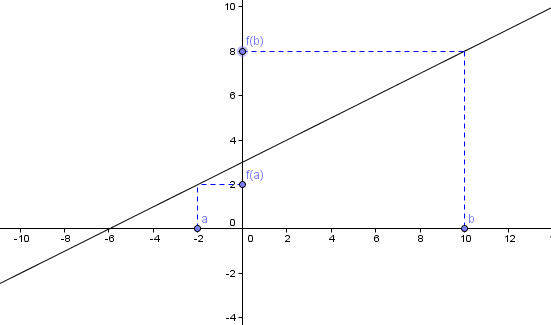
\includegraphics[scale=0.65]{./img/croiss}
		\end{center}
		
		\begin{itemize}
			\item $a$ et $b$ appartiennent à $\intervOO{- \infty }{+ \infty}$, on a $a \leq b$ donc $f(a) \leq f(b)$.
			\item $-2 \leq 10$ donc $f(-2) \leq f(10)$ ($2 \leq 8$).
		\end{itemize}
		
\end{myex}
	
	
	\subsection{Fonction décroissante}
	
	\begin{mydef}
		Si une fonction $f$ est \kw{décroissante} sur un intervalle $I$ alors les images sont rangées dans l'ordre inverse de leur antécédent ; c'est à dire que \kw{$f(x)$ diminue quand $x$ augmente}.
		
		%Si $f(x)$ augmente quand $x$ augmente, alors $f$ est \kw{croissante}.
		%Si $f(x)$ diminue quand $x$ augmente, alors $f$ est \kw{décroissante}.
	\end{mydef}
	
		\begin{myex}
		La fonction $f(x) = -x + 1$ est décroissante sur $\intervOO{- \infty }{+ \infty}$.
		\begin{center}
			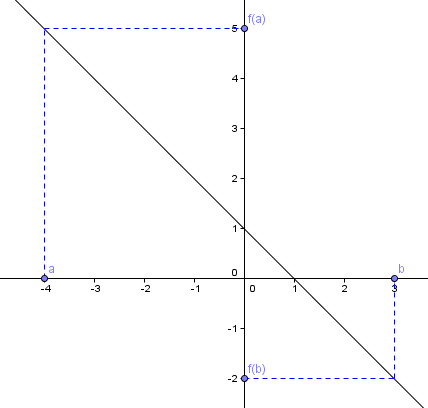
\includegraphics[scale=0.65]{./img/decroiss}
		\end{center}
		
		\begin{itemize}
			\item $a$ et $b$ appartiennent à $\intervOO{- \infty }{+ \infty}$, on a $a \leq b$ donc $f(a) \geq f(b)$.
			
			\item $-4 \leq 3$ donc $f(-4) \geq f(3)$ ($5 \geq -2 $).
		\end{itemize}
		
	\end{myex}
	
	
	\subsection{Fonction paire}
	
	\begin{mydef}
		Si une fonction $f$ est \kw{paire} sur un intervalle I, alors pour tout $x$ de I \kw{$f(-x) = f(x)$} . 
	\end{mydef}
	
	\begin{myex}
		La fonction $f(x) = |x| $ (valeur absolue de x) est définie et paire sur $\intervOO{- \infty}{+ \infty} $.
		
		\begin{center}
			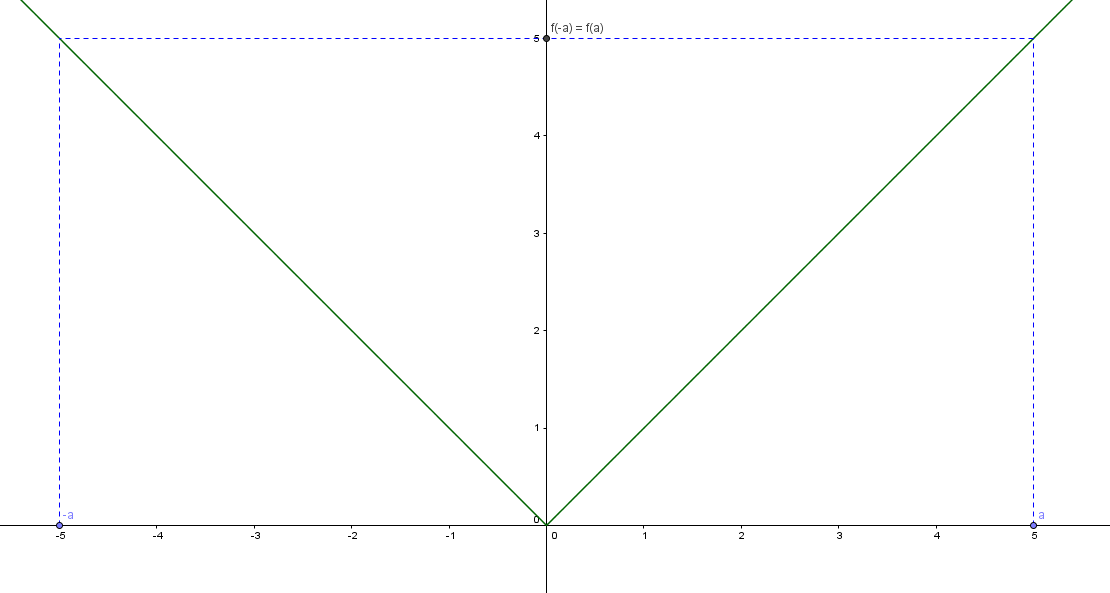
\includegraphics[scale=0.45]{img/paire}
		\end{center}
		
		On a $f(-5) = f(5) = 5$.
	\end{myex}
	
	\subsection{Fonction impaire}
	
	\begin{mydef}
		Si une fonction $f$ est \kw{impaire} sur un intervalle I, alors pour tout $x$ de I on a \kw{$f(-x) = -f(x)$} . 
	\end{mydef}
	
		\begin{myex}
		La fonction $f(x) = x $  est définie et impaire sur $\intervOO{- \infty}{+ \infty} $.
		
		\begin{center}
			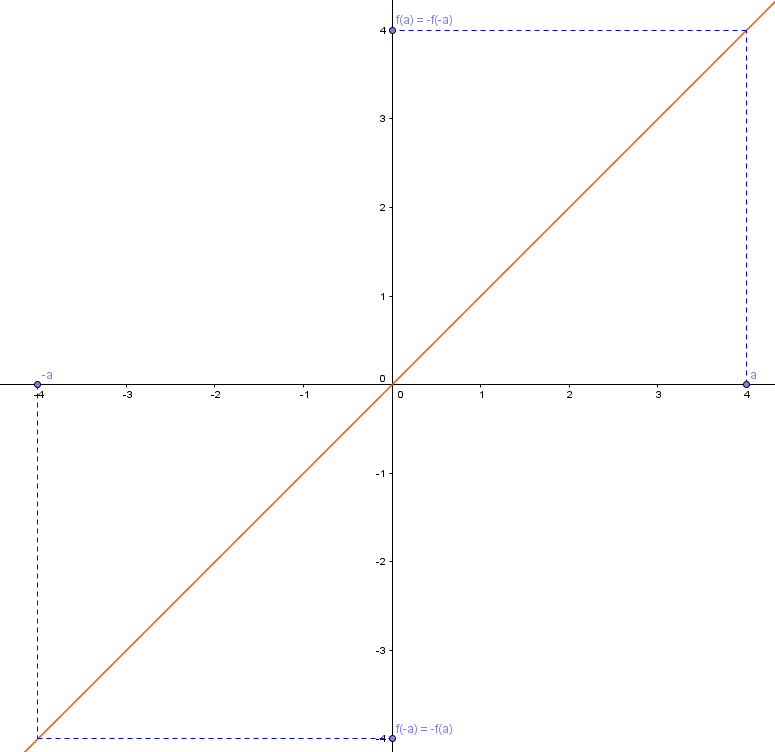
\includegraphics[scale=0.4]{img/impaire}
		\end{center}
		
		On a $f(-4) = -f(4) = -4$.
	\end{myex}
	
	%\newpage
	
	\section{Fonctions de référence}
	
	\subsection{Fonction carré}
	
	\begin{mydef}
		La \kw{fonction carré} est définie par $x \mapsto x^2$.
	\end{mydef}
	
	\begin{myprops}
		La fonction carré est :
		\begin{itemize}
			\item définie sur $\intervOO{- \infty }{+ \infty}$.
			\item décroissante sur $\intervOF{- \infty}{0}$ et croissante sur $\intervFO{0}{+ \infty}$.
			\item paire.
			%			\item Sa représentation graphique est une \kw{parabole}.
		\end{itemize}
		
	\end{myprops}
	
	
	\section{Bonus : Figure incomplète (3 points) }

$ABCD$ est un carré qui a été en partie effacé. On veut tracer son symétrique par rapport au point $O$.

\begin{questions}
	\question[1] Sans compléter le carré $ABCD$, construire $A'B'C'D'$, son symétrique par raport à $O$.
	
	\question[2] \'Ecrire un programme de construction pour $A'B'C'D'$.
\end{questions}

\begin{center}
	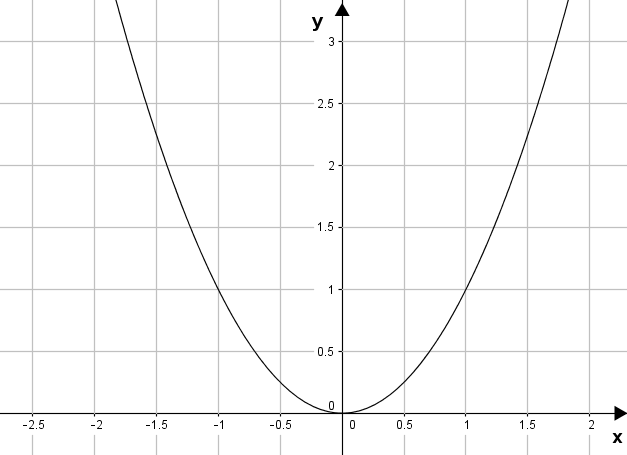
\includegraphics[scale=0.3]{img/carre}
\end{center}
	
	\subsection{Fonction inverse}
	
	\begin{mydef}
		La \kw{fonction inverse} est définie par $x \mapsto \dfrac{1}{x}$.			
	\end{mydef}
	
	\begin{myprops}
		La fonction inverse est :
		\begin{itemize}
			\item définie sur $\intervOO{-\infty}{0} \cup \intervOO{0}{+\infty}$.
			\item décroissante sur $\intervOO{- \infty}{0}$ et sur $\intervOO{0}{+ \infty}$. 
			%			\item Sa représentation graphique est une \kw{hyperbole}.
		\end{itemize}
	\end{myprops}
	
	\begin{myillus}

		Courbe représentative de la fonction $f(x) = \dfrac{1}{x}$ et tableau de variations associé:
	\begin{multicols}{2}

	


	\begin{center}
		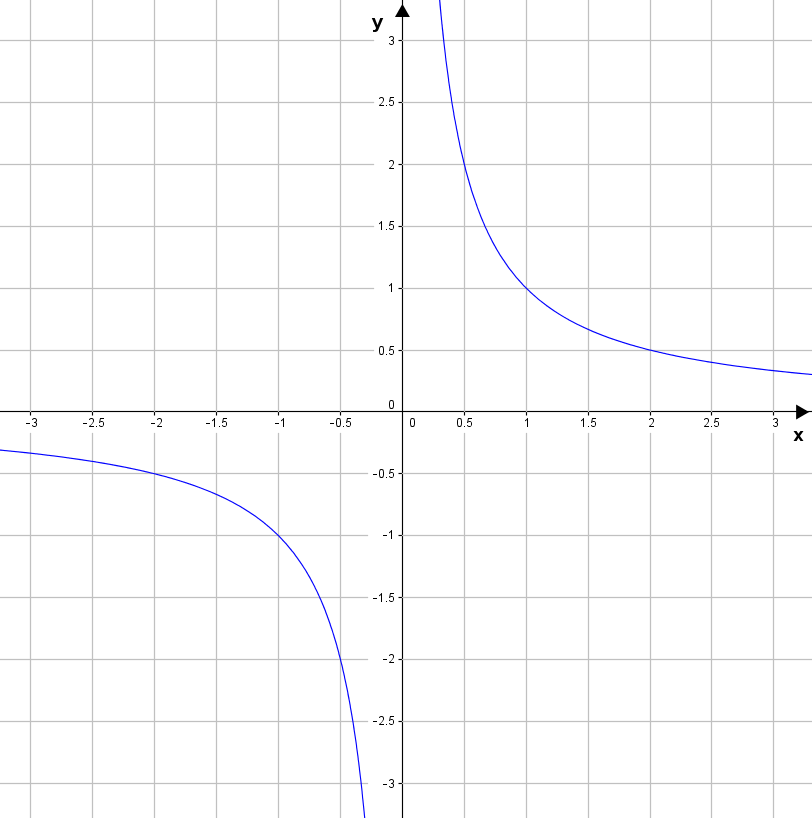
\includegraphics[scale=0.45]{./img/inverse}
	\end{center}
	
	

	\vspace*{1cm}
	\begin{center}
%		\begin{tikzpicture}
%		\tkzTabInit{$x$/1,$f(x)$/2}{$- \infty$,$0$,$+ \infty$}
%		%\tkzTabLine{,-,z,+}
%		\tkzTabVar{+/$+ \infty$,-/$0$,+/$+ \infty$}
%		\end{tikzpicture}	

		\begin{variations}
			x & \mI & & & 0 & & & \pI \\
		\filet
			\m{\dfrac{1}{x}} & \h\ & \d & \ & \bb & \h\ & \d & \ \\				
		\end{variations}
	\end{center}
	\end{multicols}
\end{myillus}
	\subsection{Fonction racine}
	
	\begin{mydef}
		La \kw{fonction racine carrée} est définie par $x \mapsto \sqrt{x}$.			
	\end{mydef}
	
	\begin{myprops}
		
		Elle est définie et croissante sur $\intervFO{0}{+\infty}$.
		
		
	\end{myprops}
	
	%\begin{myillus}

		Courbe représentative de la fonction $f(x) = \sqrt{x}$ et tableau de variations associé:
	\begin{multicols}{2}

	


	\begin{center}
		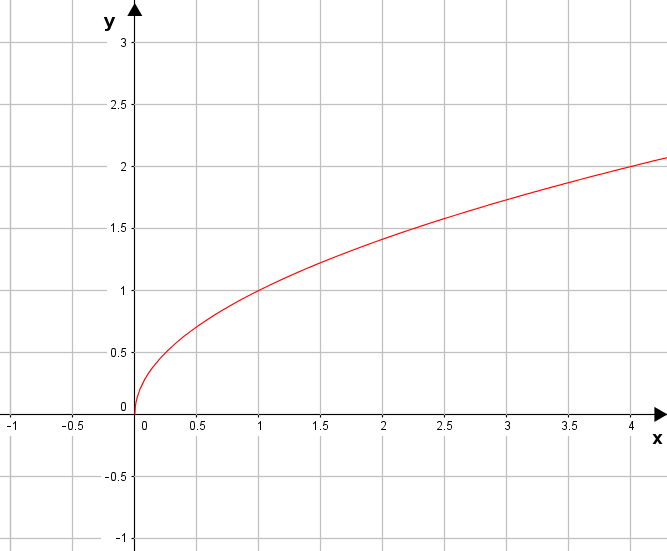
\includegraphics[scale=0.6]{./img/racine}
	\end{center}
	
	

	\vspace*{1cm}
	\begin{center}
%		\begin{tikzpicture}
%		\tkzTabInit{$x$/1,$f(x)$/2}{$- \infty$,$0$,$+ \infty$}
%		%\tkzTabLine{,-,z,+}
%		\tkzTabVar{+/$+ \infty$,-/$0$,+/$+ \infty$}
%		\end{tikzpicture}	

	\begin{variations}
		x & 0 & &  & & \pI \\
		\filet
		\sqrt{x} & & + &  \\				
	\end{variations}

	\vspace*{0.5cm}

		\begin{variations}
			x & & 0 & & \pI \\
		\filet
			\m{\sqrt{x}} & & \ & \c & \h\ \\				
		\end{variations}
	\end{center}
	\end{multicols}
%\end{myillus}
	\subsection{Fonction cube}
	
	
	\begin{mydef}
		La \kw{fonction cube} est définie par $x \mapsto x^3$.			
	\end{mydef}
	
	\begin{myprops}
		Elle est définie et croissante sur l'intervalle $\intervOO{- \infty }{+ \infty}$.
		
		
	\end{myprops}
	
	\begin{myillus}

		Courbe représentative de la fonction $f(x) = x^3$ et tableau de variations associé:
	\begin{multicols}{2}

	


	\begin{center}
		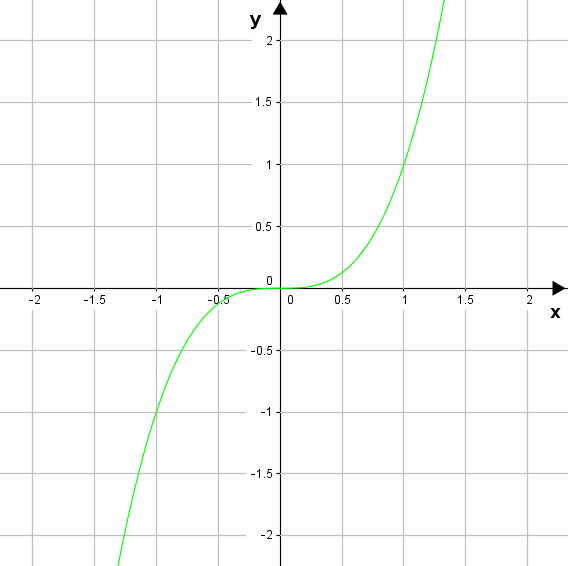
\includegraphics[scale=0.6]{./img/cube}
	\end{center}
	
	

	\vspace*{1cm}
	\begin{center}
%		\begin{tikzpicture}
%		\tkzTabInit{$x$/1,$f(x)$/2}{$- \infty$,$0$,$+ \infty$}
%		%\tkzTabLine{,-,z,+}
%		\tkzTabVar{+/$+ \infty$,-/$0$,+/$+ \infty$}
%		\end{tikzpicture}	

		\begin{variations}
			x & & \mI & & \pI \\
		\filet
			\m{x^3} & & \mI & \c & \h\pI \\				
		\end{variations}
	\end{center}
	\end{multicols}
\end{myillus}
	
	\section{Opérations avec les fonctions}
	
	\subsection{Somme d'une fonction et d'un nombre}
	
	\begin{myprop}
		Lorsque l'on \kw{ajoute une constante $k$ à  une fonction $f$}, on obtient une nouvelle fonction notée $f$+$k$ qui a \kw{le même sens de variation que $f$}.
	\end{myprop}
	
	\begin{myex}
		\begin{multicols}{2}
			\vspace*{1cm}
			
			Soit la fonction $f$, telle que $f(x) = x^2$.
			
			$f$ est décroissante sur l'intervalle $\intervOF{-\infty}{0} $ et croissante sur $\intervFO{0}{+\infty}$.
			
			Donc la fonction $f+k(x) = x^2 + 2 $ est décroissante sur l'intervalle $\intervOF{-\infty}{0} $ et croissante sur $\intervFO{0}{+\infty}$).
			
			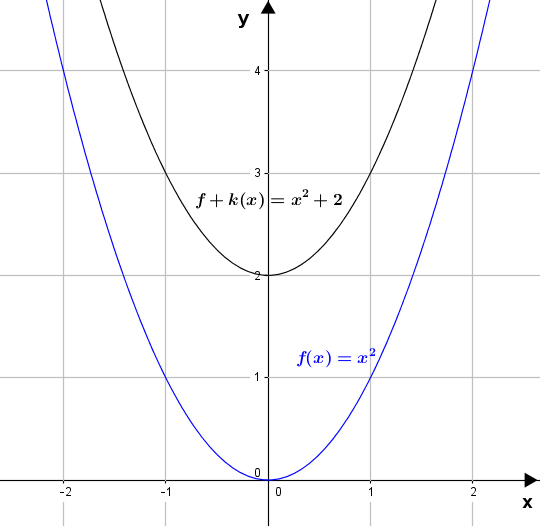
\includegraphics[scale=0.6]{./img/k+f}
		\end{multicols}
	\end{myex}
	
	\subsection{Somme de deux fonctions}
	
	\begin{myprop}
		Si on \kw{ajoute deux fonctions $f$ et $g$} qui possèdent le \kw{même sens de variation}, on obtient alors une fonction $f$+$g$ qui a \kw{le même sens de variation que $f$ ou $g$}. 
	\end{myprop}
	
	\begin{myex}
		\begin{multicols}{2}
			\vspace*{20mm}
			
			Soient les fonctions $f$ et $g$, telles que $f(x) = x^2$ et $g(x)=2x+1$.
			
			$f$ et $g$ sont croissantes sur l'intervalle $\intervFO{0}{+\infty}$.
			
			Donc la fonction $f+g(x) = x^2 + 2x + 1$ est croissante sur $\intervFO{0}{+\infty}$.
			
			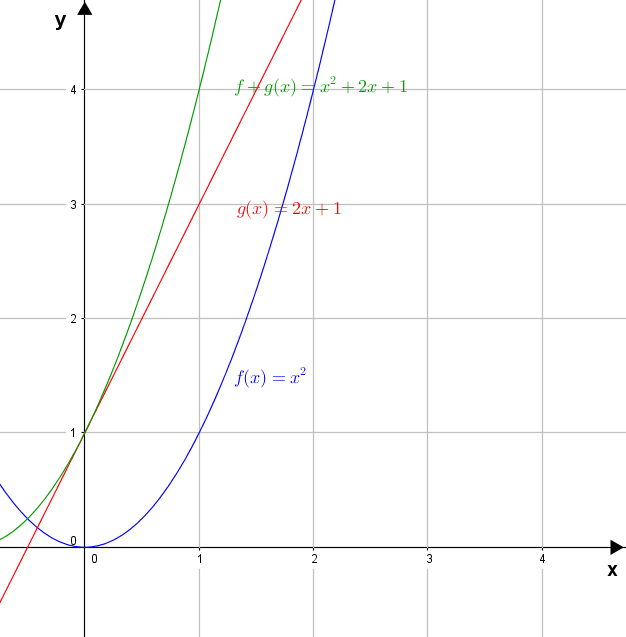
\includegraphics[scale=0.6]{./img/f+g}
		\end{multicols}
	\end{myex}
	
	\subsection{Produit d'une fonction et d'un nombre}
	
	\begin{myprops}
		\begin{itemize}
			\item Lorsque l'on \kw{multiplie une fonction $f$ par une constante  positive $k$}, on obtient alors une fonction $kf$ qui a \kw{le même sens de variation que $f$}.
			\item Lorsque l'on \kw{multiplie une fonction $f$ par une constante négative $k$}, on obtient alors une fonction $kf$ qui \kw{varie en sens contraire de $f$}.
		\end{itemize}
	\end{myprops}
	
	\begin{myex}
		%\begin{multicols}{2}
		%	\vspace*{15mm}
		
		Soit la fonction $f$, telle que $f(x) = x^2$.
		
		$f$ est décroissante sur l'intervalle $\intervOF{-\infty}{0} $ et croissante sur $\intervFO{0}{+\infty}$.
		
		Donc la fonction $kf(x) = 0,5 \times x^2$ est décroissante sur l'intervalle $\intervOF{-\infty}{0} $ et croissante sur $\intervFO{0}{+\infty}$.
		
		\begin{center}
			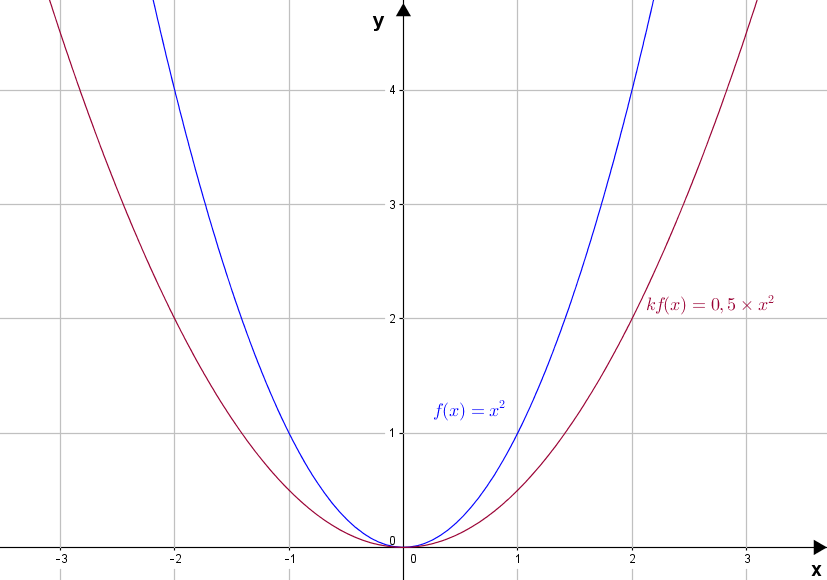
\includegraphics[scale=0.6]{./img/kf1}			
		\end{center}
		
		%\end{multicols}
	\end{myex}
	
	\begin{myex}	
		
		\begin{multicols}{2}
			\vspace*{15mm}
			
			Soit la fonction $f$, telle que $f(x) = x^2$.
			$f$ est décroissante sur l'intervalle $\intervOF{-\infty}{0} $ et croissante sur $\intervFO{0}{+\infty}$ .
			Donc la fonction $kf(x) = -2 \times x^2$ est croissante sur l'intervalle $\intervOF{-\infty}{0} $ et décroissante sur $\intervFO{0}{+\infty}$.
			
			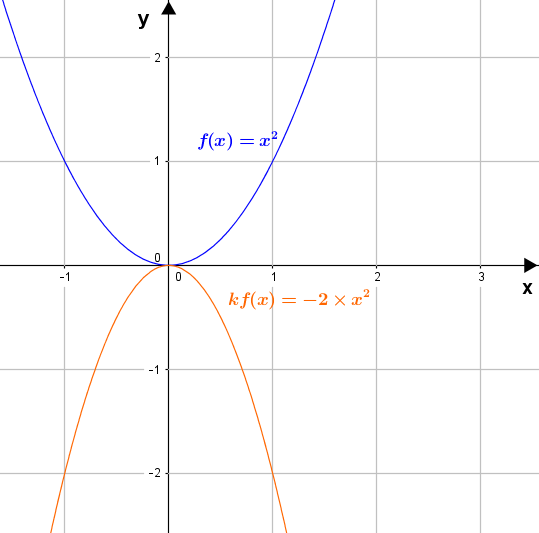
\includegraphics[scale=0.65]{./img/kf2}
		\end{multicols}
	\end{myex}
	
\end{document}